%%%%%%%%%% Page 3 - Col 1 %%%%%%%%%%
\newpage
\colorfulheader{computer graphics}

\vspace{-0.5cm}
\begin{minipage}[t]{\textwidth}
    \begin{customcenter}[5pt]
        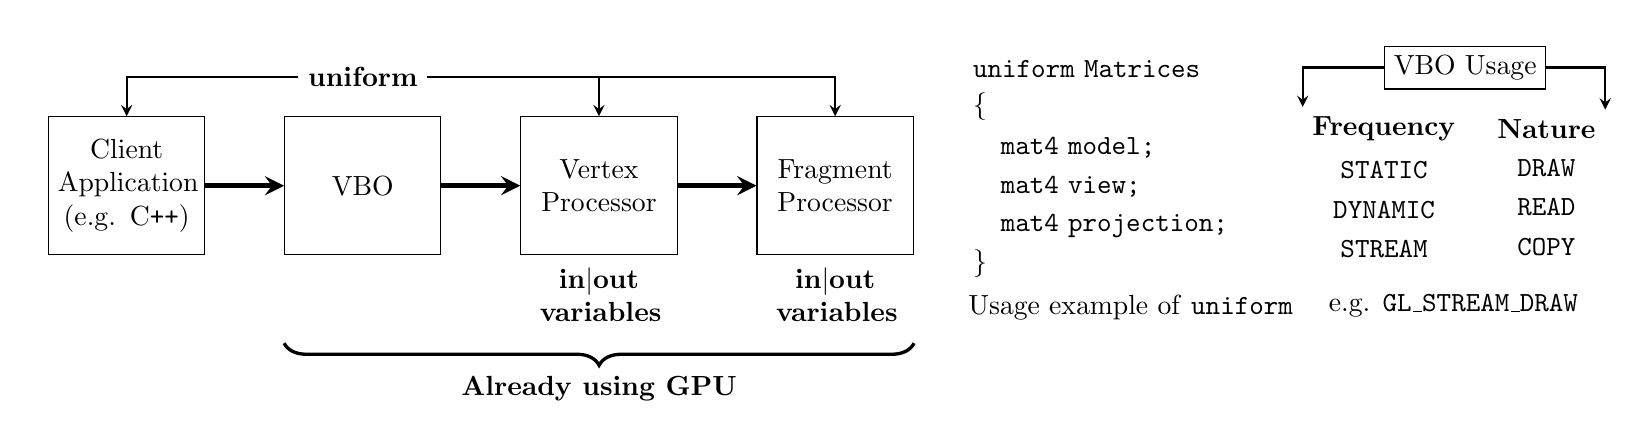
\begin{tikzpicture}
            \tikzstyle{arrow}=[thick,->,>=stealth]
            \tikzstyle{diagramnode} = [draw,text width=1.75cm,text centered,minimum height=1.75cm] 
            \tikzstyle{rowcode} = [text height=0.25cm,text width=4cm] 
            \node[rowcode] at (14,3.5) {\texttt{uniform Matrices}};
            \node[rowcode] at (14,3.0) {\texttt{\{}};
            \node[rowcode] at (14,2.5) {\hspace{10pt}\texttt{mat4 model;}};
            \node[rowcode] at (14,2.0) {\hspace{10pt}\texttt{mat4 view;}};
            \node[rowcode] at (14,1.5) {\hspace{10pt}\texttt{mat4 projection;}};
            \node[rowcode] (matnode) at (14,1.0) {\texttt{\}}};
            \node[yshift=-0.25cm] at (matnode.south) {Usage example of \texttt{uniform}};
            \node[draw] (vbousagenode) at (18.25,3.5) {VBO Usage};
            \node[yshift=-0.5cm] (f) at (vbousagenode.south west) {\textbf{Frequency}};
            \node[yshift=-0.5cm] (n) at (vbousagenode.south east) {\textbf{Nature}};
            \node[yshift=-0.25cm] () at (f.south) {\texttt{STATIC}};
            \node[yshift=-0.75cm] () at (f.south) {\texttt{DYNAMIC}};
            \node[yshift=-1.25cm] () at (f.south) {\texttt{STREAM}};
            \node[yshift=-0.25cm] () at (n.south) {\texttt{DRAW}};
            \node[yshift=-0.75cm] () at (n.south) {\texttt{READ}};
            \node[yshift=-1.25cm] () at (n.south) {\texttt{COPY}};
            \node[yshift=-2.75cm,xshift=-0.15cm] () at (vbousagenode.south) {e.g. \texttt{GL\_STREAM\_DRAW}};
            \draw[arrow] (vbousagenode.west) -| (f.north west);
            \draw[arrow] (vbousagenode.east) -| (n.north east);
            \draw[step=1cm,black,thin,transparent] (0,0) grid (20,4);
            \node[diagramnode] (start) at (1.25,2) {Client \\ Application \\ (e.g. C\texttt{++})};
            \node[diagramnode,xshift=2cm] (vbonode) at (start.east) {VBO};
            \node[diagramnode,xshift=2cm] (vertexnode) at (vbonode.east) {Vertex \\ Processor};
            \node[diagramnode,xshift=2cm] (fragmentnode) at (vertexnode.east) {Fragment \\ Processor};
            \node[yshift=0.5cm] (uniformnode) at (vbonode.north) {\textbf{uniform}};
            \node[yshift=-0.5cm,text centered,text width=1.5cm] at (vertexnode.south) {\textbf{in$|$out \\ variables}};
            \node[yshift=-0.5cm,text centered,text width=1.5cm] at (fragmentnode.south) {\textbf{in$|$out \\ variables}};
            \draw[arrow,line width=2pt] (start) -- (vbonode);
            \draw[arrow,line width=2pt] (vbonode) -- (vertexnode);
            \draw[arrow,line width=2pt] (vertexnode) -- (fragmentnode);
            \draw[arrow] (uniformnode) -| (start);
            \draw[arrow] (uniformnode) -| (vertexnode);
            \draw[arrow] (uniformnode) -| (fragmentnode);
            \draw[decorate,decoration={brace,mirror,amplitude=8pt},very thick] (3.25,0.00) -- (11.25,0.00) node[black,pos=0.5,below=8pt,anchor=north]{\textbf{Already using GPU}};
        \end{tikzpicture}
    \end{customcenter}
\end{minipage}

\hspace{-5pt}
\begin{minipage}[t]{0.585\textwidth}
    \begin{customcenter}[5pt]
        \textbf{Client Side (CPU)}
        \begin{tikzpicture}[background rectangle/.style={fill=blue!10}, show background rectangle]
            \tikzstyle{arrow}=[thick,->,>=stealth]
            \tikzstyle{rowcode} = [text height=0.25cm,text width=10cm] 
            \draw[step=1cm,blue!10,very thin] (0,0) grid (12,-10);
            \draw[decorate,decoration={brace,mirror,amplitude=8pt},very thick] (0.00,0.25) -- (0.00,-7.75) node[black,pos=0.5,rotate=90,below=-8pt,anchor=south]{\textbf{INITIALIZATION}};
            \draw[decorate,decoration={brace,mirror,amplitude=8pt},very thick] (0.00,-7.75) -- (0.00,-9.75) node[black,pos=0.5,rotate=90,below=-8pt,anchor=south]{\textbf{DISPLAY}};
            \node[rowcode] at (5,+0.0) {\texttt{GLint vao;}};
            \node[rowcode] at (5,-0.5) {\texttt{glGenVertexArray(1,\&vao);}};
            \node[rowcode] at (5,-1.0) {\texttt{glBindVertexArray(vao);}};
            \node[rowcode] at (5,-1.5) {\texttt{GLfloat ** data = ... \textbackslash\textbackslash Initialize data;}};
            \node[rowcode] at (5,-2.0) {\texttt{glBindBuffer(GL\_ARRAY\_BUFFER,vbo);}};
            \node[rowcode] at (5,-2.5) {\texttt{glBufferData(GL\_ARRAY\_BUFFER,sizeof(data),data,GL\_STATIC\_DRAW);}};
            \node[xshift=-2.25cm] (vs) at (5, -3.25) {\footnotesize\texttt{\{GL\_VERTEX\_SHADER,"vs.glsl",}};
            \node[xshift=+1.95cm] (fs) at (5, -3.25) {\footnotesize\texttt{GL\_FRAGMENT\_SHADER,"fs.glsl"\}}};
            \node[rowcode] (shaderfunc) at (5,-4.0) {\texttt{GLuint programID = LoadShader(}\textbf{vertex}\texttt{,}\textbf{fragment}\texttt{);}};
            \draw[decorate,decoration={brace,amplitude=8pt},thick] (5.55,-3.75) -- (8.35,-3.75);
            \node[rowcode] at (5,-4.5) {\texttt{glUseProgram(programID);}};
            \node at (3.8,-5.25) {\tiny{$\substack{\text{VERTEX SHADER}\\\text{POSITION}}$}};
            \node at (4.5,-6.75) {\tiny{$\substack{\text{PER VERTEX}\\\text{\# ELEMENTS}}$}};
            \node at (5.5,-5.25) {\tiny{$\substack{\text{DATA}\\\text{TYPE}}$}};
            \node at (7.0,-6.75) {\tiny{$\substack{\text{DATA}\\\text{NORMALIZATION}}$}};
            \node at (8.1,-5.25) {\tiny{$\substack{\text{DATA}\\\text{STRIDE}}$}};
            \node at (9.0,-6.75) {\tiny{$\substack{\text{POINTER TO}\\\text{INIT MEMORY}}$}};
            \node[rowcode] at (5,-6.0) {\texttt{glVertexAttribPointer(0,2,GL\_FLOAT,GL\_FALSE,0,nullptr);}};
            \draw[arrow] (4.125,-5.75) -- (4.125,-5.5);
            \draw[arrow] (5.500,-5.75) -- (5.500,-5.5);
            \draw[arrow] (8.100,-5.75) -- (8.100,-5.5);
            \draw[arrow] (4.500,-6.20) -- (4.500,-6.5);
            \draw[arrow] (7.000,-6.20) -- (7.000,-6.5);
            \draw[arrow] (9.000,-6.20) -- (9.000,-6.5);
            \node[rowcode] at (5,-7.5) {\texttt{glEnableVertexAttribArray(0);}};
            \node[rowcode] at (5,-8.0) {\texttt{glClear(GL\_COLOR\_BUFFER\_BIT);}};
            \node[rowcode] at (5,-8.5) {\texttt{glBindVertexArray(vao);}};
            \node[rowcode] at (5,-9.0) {\texttt{glDrawArrays(GL\_TRIANGLES,0,}\textbf{number of vertices}\texttt{)};};
            \node[rowcode] at (5,-9.5) {\texttt{glSwapBuffers();}};
        \end{tikzpicture}
    \end{customcenter}
\end{minipage}
\hspace{5pt}
\begin{minipage}[t]{0.35\textwidth}
    \begin{customcenter}[5pt]
        \textbf{Server Side (GPU)}
        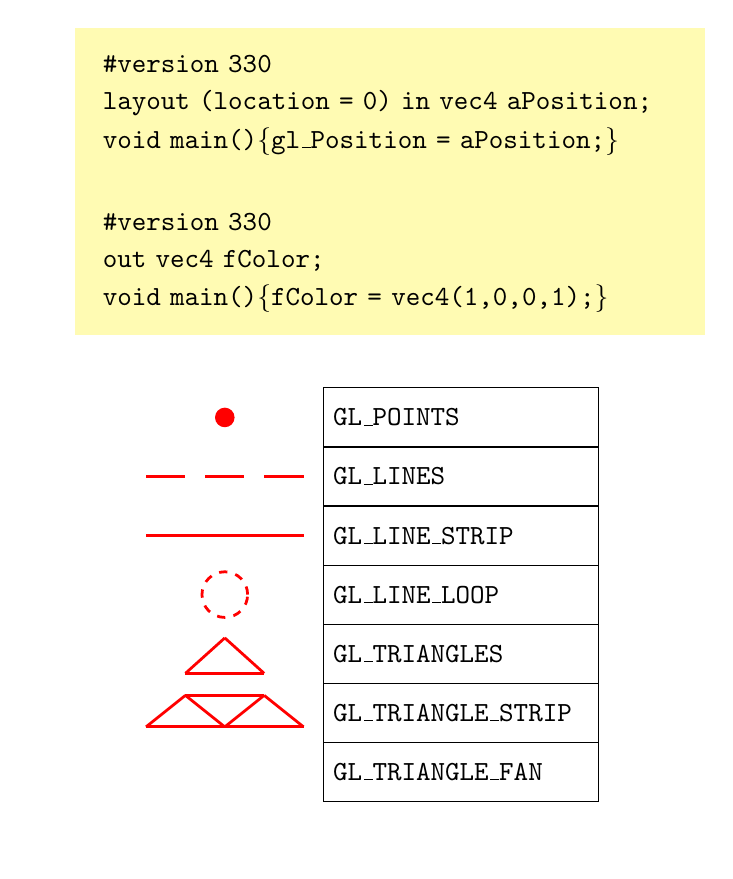
\begin{tikzpicture}        
            \begin{scope}[xshift=0.95cm]
                \tikzstyle{rowcodeshader} = [text height=0.25cm,text width=7.5cm] 
                \node[rectangle,fill=yellow!30,minimum width=8.0cm,minimum height=3.9cm] at (3.65,-1.5){};
                \node[rowcodeshader] at (3.75,+0.0) {\texttt{\#version 330}};
                \node[rowcodeshader] at (3.75,-0.5) {\texttt{layout (location = 0) in vec4 aPosition;}};
                \node[rowcodeshader] at (3.75,-1.0) {\texttt{void main()\{gl\_Position = aPosition;\}}};
                \node[rowcodeshader] at (3.75,-2.0) {\texttt{\#version 330}};
                \node[rowcodeshader] at (3.75,-2.5) {\texttt{out vec4 fColor;}};
                \node[rowcodeshader] at (3.75,-3.0) {\texttt{void main()\{fColor = vec4(1,0,0,1);\}}};
            \end{scope}
            \draw[step=1cm,black,very thin,transparent] (0,0) grid (8,-10);
            \begin{scope}[xshift=0.75cm]
                \tikzstyle{nodetype} = [anchor=west,text width=3.25cm,draw,minimum height=0.75cm]
                \node[nodetype]() at (3,-4.50) {\texttt{GL\_POINTS}};
                \node[nodetype]() at (3,-5.25) {\texttt{GL\_LINES}};
                \node[nodetype]() at (3,-6.00) {\texttt{GL\_LINE\_STRIP}};
                \node[nodetype]() at (3,-6.75) {\texttt{GL\_LINE\_LOOP}};
                \node[nodetype]() at (3,-7.50) {\texttt{GL\_TRIANGLES}};
                \node[nodetype]() at (3,-8.25) {\texttt{GL\_TRIANGLE\_STRIP}};
                \node[nodetype]() at (3,-9.00) {\texttt{GL\_TRIANGLE\_FAN}};
                \node[scale=0.75,circle,fill=red] at (1.75,-4.50) {};
                \draw[red,line width=1pt] (0.75,-5.25) -- (1.25,-5.25) {};
                \draw[red,line width=1pt] (1.50,-5.25) -- (2.00,-5.25) {};
                \draw[red,line width=1pt] (2.25,-5.25) -- (2.75,-5.25) {};
                \draw[red,line width=1pt] (0.75,-6.00) -- (2.75,-6.00) {};
                \node[scale=1.75,circle,draw=red,dashed,line width=1pt] at (1.75,-6.75) {};
                \draw[red,line width=1pt] (1.75,-7.30) -- (1.25,-7.75) {};
                \draw[red,line width=1pt] (1.75,-7.30) -- (2.25,-7.75) {};
                \draw[red,line width=1pt] (1.25,-7.75) -- (2.25,-7.75) {};
                \begin{scope}[yshift=2pt]
                    \draw[red,line width=1pt] (1.25,-8.1) -- (0.75,-8.5) {};
                    \draw[red,line width=1pt] (1.25,-8.1) -- (1.75,-8.5) {};
                    \draw[red,line width=1pt] (0.75,-8.5) -- (1.75,-8.5) {};
                    \draw[red,line width=1pt] (1.25,-8.1) -- (2.25,-8.1) {};
                    \draw[red,line width=1pt] (1.75,-8.5) -- (2.25,-8.1) {};
                    \draw[red,line width=1pt] (2.25,-8.1) -- (2.75,-8.5) {};
                    \draw[red,line width=1pt] (1.75,-8.5) -- (2.75,-8.5) {};
                \end{scope}
            \end{scope}
        \end{tikzpicture}
    \end{customcenter}
\end{minipage}
\emptyline

\begin{minipage}[t]{0.55\textwidth}
    \colorfulsection{Ray Tracing}
    \begin{itemize}[leftmargin=*]
        \setlength\itemsep{0pt}
        \item A color in the computer needs the \textbf{discretization mapping} $f = \left[0, 1\right)\mapsto\bracketA{0, \dots, 255} = i$, which can be achieved by $i = $\texttt{int}$\parenthesisA{256\times f}$
        \item Due to \textbf{non-linearity on screens} ($i\hspace{-2pt}=\hspace{-2pt}128$ is not half as bright as $i\hspace{-2pt}=\hspace{-2pt}255$) one might do a \textbf{gamma correction} $i = \text{\texttt{int}}\hspace{-2pt}\parenthesisA{256 \times f^{\frac{1}{\gamma}}}$
        \item The \textbf{parameter gamma} $\gamma$ is characterized by system but ranges from 1.7 to 2.3. For example, Linux and PCs use 2.2 while Macintosh uses 1.8
        \item Given the ray $\mathcal{R} = \mathbf{o} + t\mathbf{d},\; t\in\left[0,\infty\right)$, some closed solutions for \textbf{intersection surface-ray} are
        \begin{customcenter}[0pt]
            \begin{tabular}{|l|c|}
                \hline
                Surface & \textbf{Intersection }\parenthesis{value of $t$}\\
                \hline
                \multirow{2}{*}{\textit{Plane} $\mapsto$ $\parenthesisA{\mathbf{p} - \mathbf{a}}\cdot\mathbf{n} = 0$} & \multirow{2}{*}{$\frac{\parenthesisA{\mathbf{a} - \mathbf{o}}\cdot\mathbf{n}}{\mathbf{d}\cdot\mathbf{n}}$} \\
                & \\
                \hline
                \multirow{2}{*}{\textit{Sphere} $\mapsto$ $\norm{\mathbf{p} - \mathbf{c}}^2 - r^2 = 0$} & \multirow{2}{*}{$\frac{-\mathbf{d}\cdot\mathbf{b}\pm\bracketA{\parenthesisA{\mathbf{d}\cdot\mathbf{b}}^2 - \norm{\mathbf{d}}^2\parenthesisA{\norm{\mathbf{b}}^2 - r^2}}}{\norm{\mathbf{u}}^2}^{\frac{1}{2}}\begin{aligned}\mathbf{b} = \parenthesisA{\mathbf{o}-\mathbf{c}}\end{aligned}$} \\
                & \\
                \hline
                & \\[-8pt]
                \textit{Triangle} & \\[-3pt]
                $\begin{aligned}\mathbf{p}_{\alpha\beta\gamma} &= \alpha\mathbf{a}\hspace{-2pt}+\hspace{-2pt}\beta\mathbf{b}\hspace{-2pt}+\hspace{-2pt}\gamma\mathbf{c}\\ &\hspace{-14pt}\underset{\alpha + \beta + \gamma = 1}{=}\hspace{-14pt}\mathbf{a}\hspace{-2pt}+\hspace{-2pt}\beta\parenthesisA{\mathbf{b}\hspace{-2pt}-\hspace{-2pt}\mathbf{a}}\hspace{-2pt}+\hspace{-2pt}\gamma\parenthesisA{\mathbf{c}\hspace{-2pt}-\hspace{-2pt}\mathbf{a}}\end{aligned}$ & $\begin{bmatrix} \uparrow & \hspace{-8pt}\uparrow & \hspace{-8pt}\uparrow \\ \parenthesisA{\mathbf{a} - \mathbf{b}} & \hspace{-8pt}\parenthesisA{\mathbf{a} - \mathbf{c}} & \hspace{-8pt}\mathbf{d} \\ \downarrow & \hspace{-8pt}\downarrow & \hspace{-8pt}\downarrow \end{bmatrix}\begin{bmatrix}\beta \\ \gamma \\ t\end{bmatrix}\hspace{-2pt}=\hspace{-2pt}\begin{bmatrix}\uparrow\\\parenthesisA{\mathbf{a} - \mathbf{o}}\\\downarrow\end{bmatrix}$ \\
                & $\beta + \gamma < 1,\;\beta > 0,\;\gamma > 0$\\ 
                \hline
            \end{tabular}
        \end{customcenter}
        \end{itemize}    
\end{minipage}
